\documentclass[a4paper,14pt]{extreport}
\usepackage[left=1.5cm,right=1.5cm,
    top=1.5cm,bottom=2cm,bindingoffset=0cm]{geometry}
\usepackage{scrextend}
\usepackage[T1,T2A]{fontenc}
\usepackage[utf8]{inputenc}
\usepackage[english,russian,ukrainian]{babel}
\usepackage{tabularx}
\usepackage{amssymb}
\usepackage{color}
\usepackage{amsmath}
\usepackage{mathrsfs}
\usepackage{listings}
\usepackage{graphicx}
\graphicspath{ {./images/} }
\usepackage{lipsum}
\usepackage{xcolor}
\usepackage{hyperref}
\usepackage{tcolorbox}
\usepackage{tikz}
\usepackage[framemethod=TikZ]{mdframed}
\usepackage{wrapfig,boxedminipage,lipsum}
\mdfdefinestyle{MyFrame}{%
linecolor=blue,outerlinewidth=2pt,roundcorner=20pt,innertopmargin=\baselineskip,innerbottommargin=\baselineskip,innerrightmargin=20pt,innerleftmargin=20pt,backgroundcolor=gray!50!white}
 \usepackage{csvsimple}
 \usepackage{supertabular}
\usepackage{pdflscape}
\usepackage{fancyvrb}
%\usepackage{comment}
\definecolor{ggreen}{rgb}{0.4,1,0}
\definecolor{rred}{rgb}{1,0.1,0.1}
\usepackage{array,tabularx}
\usepackage{colortbl}

\usepackage{varwidth}
\tcbuselibrary{skins}
\usepackage{fancybox}

\definecolor{ggreen}{rgb}{0.4,1,0}
\definecolor{rred}{rgb}{1,0.1,0.1}
\definecolor{amber}{rgb}{1.0, 0.75, 0.0}
\definecolor{babyblue}{rgb}{0.54, 0.81, 0.94}
\definecolor{asparagus}{rgb}{0.53, 0.66, 0.42}
\definecolor{chartreuse}{rgb}{0.5, 1.0, 0.0}
\definecolor{darkorchid}{rgb}{0.6, 0.2, 0.8}


\usepackage{float}
\usepackage{wrapfig}
\usepackage{framed}
%for nice Code{
\lstdefinestyle{customc}{
  belowcaptionskip=1\baselineskip,
  breaklines=true,
  frame=L,
  xleftmargin=\parindent,
  language=C,
  showstringspaces=false,
  basicstyle=\small\ttfamily,
  keywordstyle=\bfseries\color{green!40!black},
  commentstyle=\itshape\color{purple!40!black},
  identifierstyle=\color{blue},
  stringstyle=\color{orange},
}
\lstset{escapechar=@,style=customc}
%}


\begin{document}

\newtcbox{\xmybox}[1][red]{on line, arc=7pt,colback=#1!10!white,colframe=#1!50!black, before upper={\rule[3pt] {0pt}{10pt}},boxrule=1pt,boxsep=0pt,left=6pt,right=6pt,top=2pt,bottom=2pt}


\pagecolor{white}
\begin{titlepage}
  \begin{center}
    \large
    Національний технічний університет України \\ "Київський політехнічний інститут імені Ігоря Сікорського"


    Факультет Електроніки

    Кафедра мікроелектроніки
    \vfill

    \textsc{ЗВІТ}\\

    {\Large Про виконання практичної роботи №2\\
      з дисципліни: «Твердотільна електроніка-2»\\[1cm]

      Діодне включення біполярного інтегрального транзистора в напівпровідникових ІМС.


    }
  \bigskip
\end{center}
\vfill

\newlength{\ML}
\settowidth{\ML}{«\underline{\hspace{0.4cm}}» \underline{\hspace{2cm}}}
\hfill
\begin{minipage}{1\textwidth}
Виконавець:\\
Студент 3-го курсу \hspace{4cm} $\underset{\text{(підпис)}}{\underline{\hspace{0.2\textwidth}}}$  \hspace{1cm}А.\,С.~Мнацаканов\\
\vspace{1cm}

Перевірив: \hspace{6.1cm} $\underset{\text{(підпис)}}{\underline{\hspace{0.2\textwidth}}}$  \hspace{1cm}О.\,В.~Мачулянський\\

\end{minipage}

\vfill

\begin{center}
2021
\end{center}
\end{titlepage}


\begin{center}ЗАВДАННЯ\end{center}

\begin{enumerate}
  \item еквівалентні схеми інтегральних діодів в біполярних ІМС;
  \item та переріз структур для наступних варіантів діодного включення ІТ:
  \begin{enumerate}
    \item перехід Б-Е з колектором, закороченим на базу;
    \item паралельне включення обох переходів.
  \end{enumerate}
\end{enumerate}

\begin{center}\fbox{\fcolorbox{black}{amber}{1}}\end{center}

\begin{figure}[h]
    \center{
\includegraphics[scale = 0.7]{1.png}}
  \caption{перехід Б-Е з колектором, закороченим на базу.}
  \label{ris1}
\end{figure}

\begin{figure}[h]
    \center{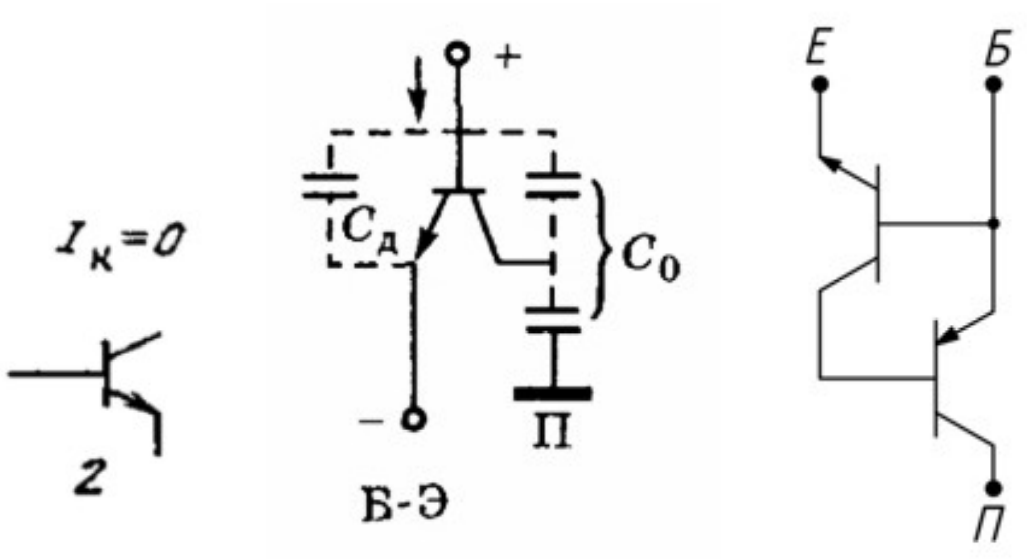
\includegraphics[scale = 0.7]{2.png}}
  \caption{перехід Б-Е з розімкнутим ланцюгом колектора.}
  \label{ris1}
\end{figure}

\begin{figure}[h]
    \center{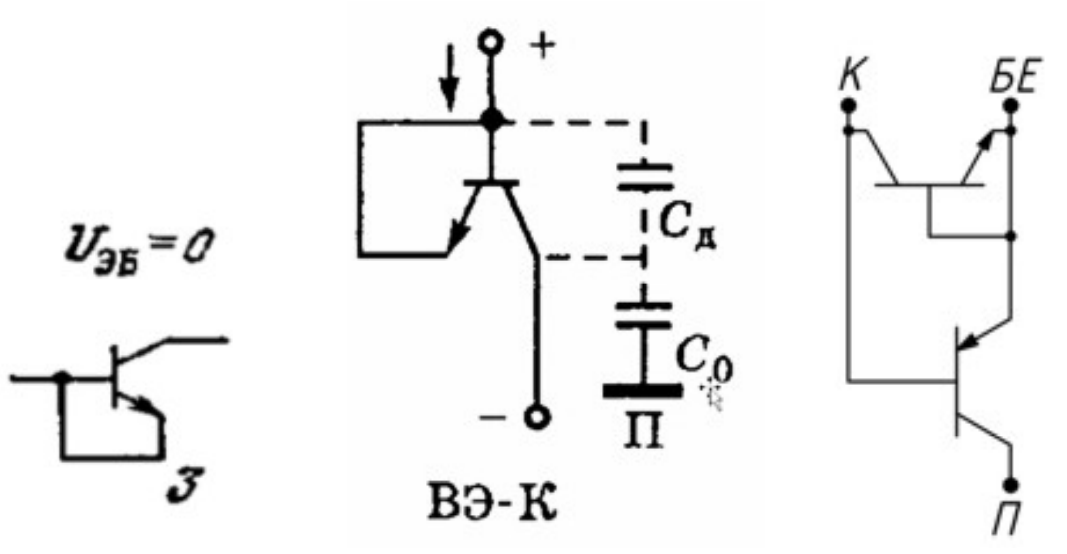
\includegraphics[scale = 0.7]{3.png}}
  \caption{перехід К-Б з емітером, закороченим на базу.}
  \label{ris1}
\end{figure}

\begin{figure}[h]
    \center{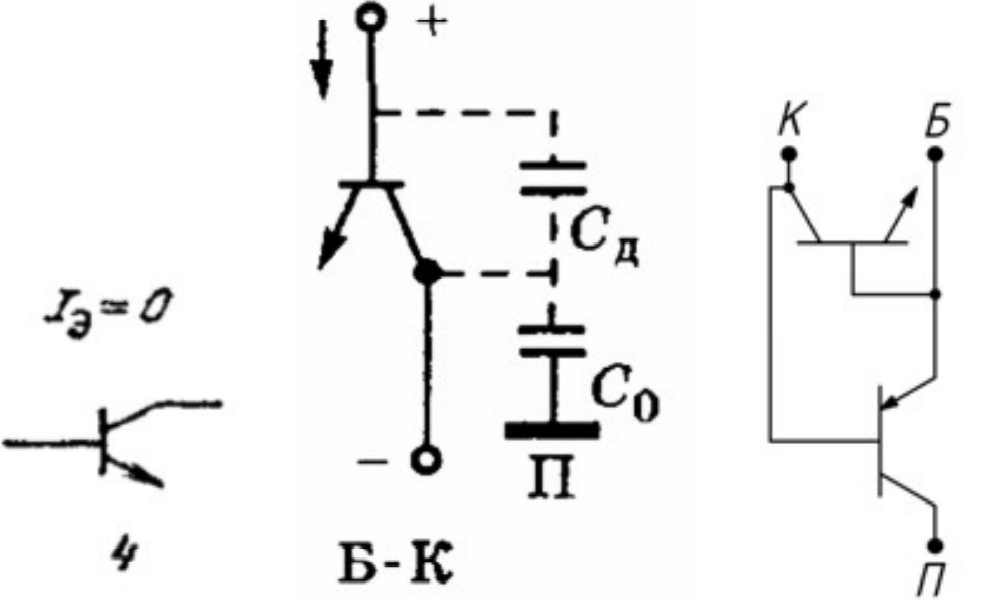
\includegraphics[scale = 0.7]{4.png}}
  \caption{перехід Б-К з розімкнутим ланцюгом емітера.}
  \label{ris1}
\end{figure}

\begin{figure}[h]
    \center{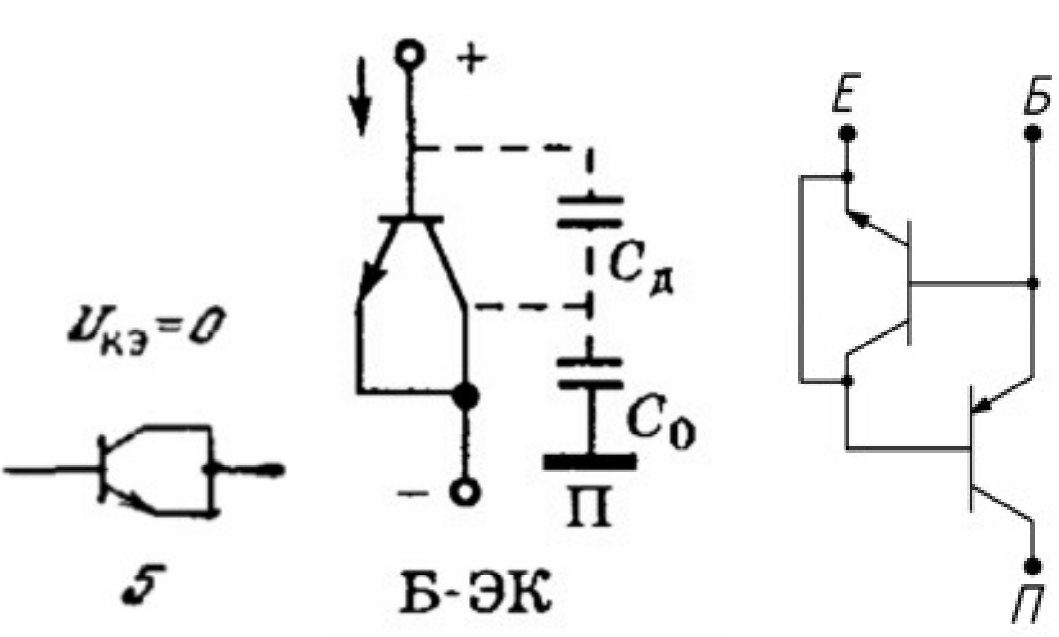
\includegraphics[scale = 0.7]{5.png}}
  \caption{паралельне включення обох переходів.}
  \label{ris1}
\end{figure}




\clearpage
\begin{center}\fbox{\fcolorbox{black}{babyblue}{2}}\end{center}


\begin{figure}[h]
    \center{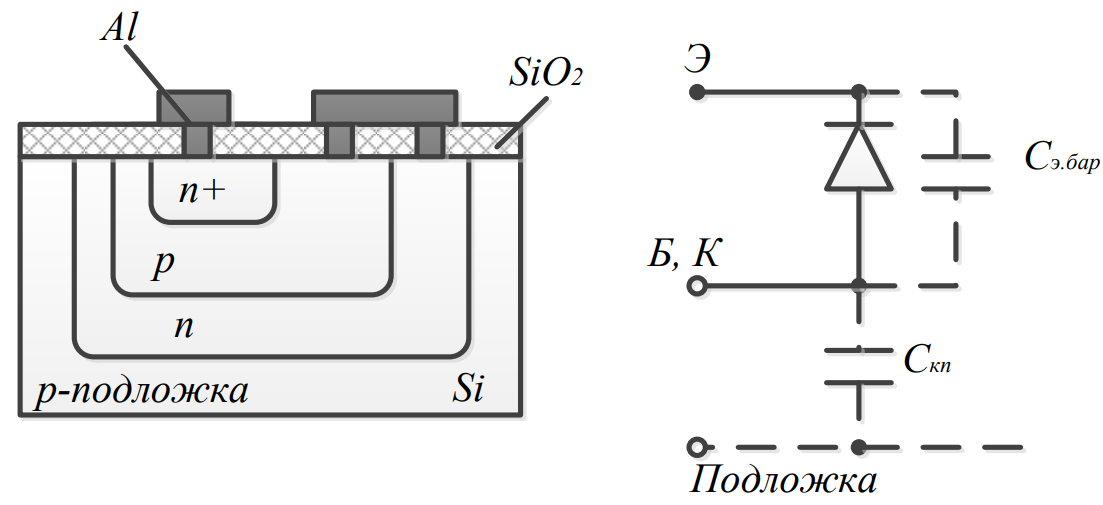
\includegraphics[scale = 0.7]{6.png}}
\end{figure}

\begin{figure}[h]
    \center{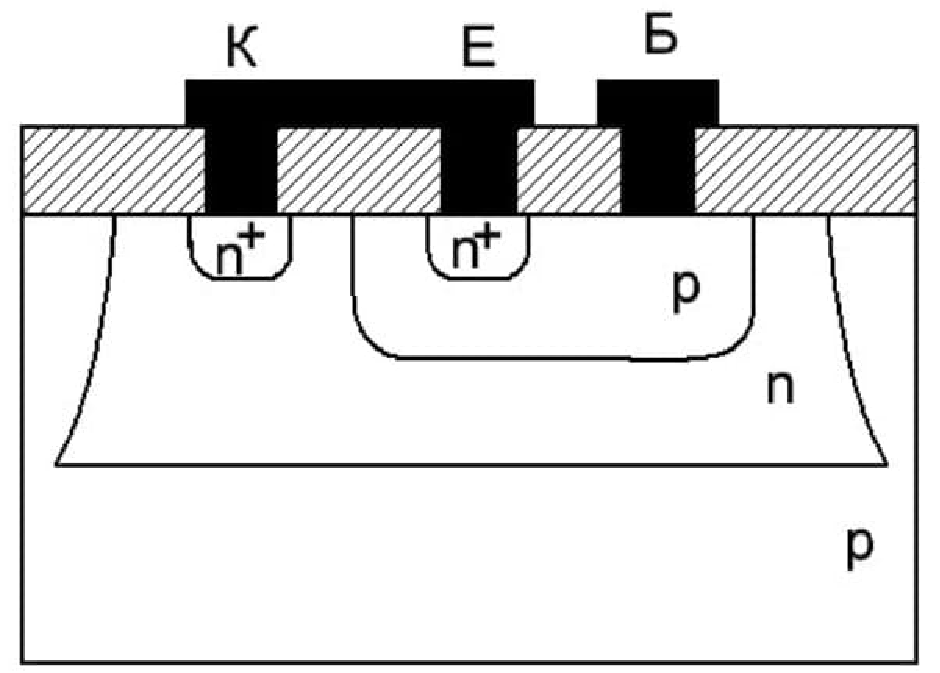
\includegraphics[scale = 0.7]{7.pdf}}


\end{figure}






















\end{document}
